\documentclass [a4paper,12pt]{article}
\usepackage{amsmath,amsthm,amssymb}
\usepackage{graphicx}
\usepackage{mathtext}
\usepackage[T1,T2A]{fontenc}
\usepackage[utf8]{inputenc}
\usepackage[english,russian]{babel}


\title{Домашние задание №1 по дисциплине "Теория случайных процессов"}

\author{Головатских Марк \\БПМ-16-1 \\ Вариант 6}
\date{}
\begin{document}

\maketitle
\pagenumbering{gobble}
\newpage
\pagenumbering{arabic}
Матрица одношаговых переходов:\\

$P = \left(
\begin{matrix}
\frac{1}{2} & \frac{1}{2} & 0 & 0&0&0&0&0\\
1 & 0 & 0 & 0&0&0&0&0&\\
0 & 0 & 0 & 0&\frac{1}{3}&0&\frac{2}{3}&0\\
0 & \frac{1}{2} & \frac{1}{2} & 0&0&0&0&0\\
0 & 0 & 0 & \frac{3}{4}&0&0&0&\frac{1}{4}\\
0 & 0 & 0 & 0&0&0&0&1\\
0 & 0 & 0 & 0&0&1&0&0\\
0 & 0 & 0 & 0&0&0&1&0\\
\end{matrix}
\right) $\\

Построим граф состояний этой марковской цепи:\\

\begin{figure}[h!]
  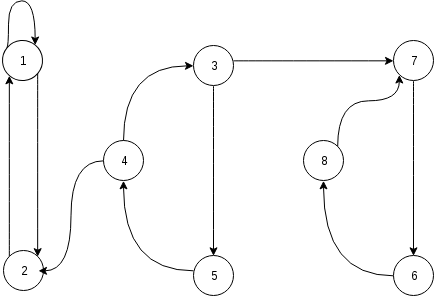
\includegraphics[width=\linewidth]{hw1.png}
\end{figure}
Разобьем все состояния на классы эквивалентности:
\{1, 2\}, \{6, 7, 8\} и \{3, 4, 5\}.\\
Рассмотрим каждый класс отдельно:\\
\section{\{1, 2\}}
Это возвратный непериодический класс.\\
Составим и решим уравнения на финальные вероятности этого класса. $x_1$ - финальная вероятность состояния $1$, $x_2$ - финальная вероятность состояния $2$.\\
\begin{equation*}
 \begin{cases}
   x_1=x_2+\frac{1}{2}x_1
   \\
   x_2 =\frac{1}{2}x_1
 \end{cases}
\end{equation*}
Финальные вероятности связаны уравнением  $x_2 + x_1 = 1$, заменим на него второе уравнение.\\
\begin{equation*}
 \begin{cases}
   x_1=x_2+\frac{1}{2}x_1
   \\
   x_2 + x_1 = 1
 \end{cases}
\end{equation*}
Решив систему получим:\\
\begin{equation*}
 \begin{cases}
   x_1=\frac{2}{3}
   \\
   x_2=\frac{1}{3}
 \end{cases}
\end{equation*}
\section{\{6, 7, 8\}}
Это периодический возвратный класс. Его период $d=3$.\\
\section{\{3, 4, 5\}}
Это невозвратный класс. Его период $d=3$. Найдем вероятность поглащения состояний этого класса классом \{1, 2\}. Обозначим за $x_i$ вероятность поглащения для $i$-ого состояния. Составим систему:\\
\begin{equation*}
 \begin{cases}
  x_3=\frac{1}{3}x_5
   \\
   x_4=\frac{1}{2} + \frac{1}{2}x_3
   \\
   x_5=\frac{3}{4}x_4
 \end{cases}
\end{equation*}
Решив систему получим:\\
\begin{equation*}
 \begin{cases}
  x_3=\frac{1}{7}
   \\
   x_4=\frac{4}{7}
   \\
   x_5=\frac{3}{7}
 \end{cases}
\end{equation*}
\end{document}
